\chapter{Conferme sperimentali della relatività speciale}
\minitoc

\section{Il decadimento dei mesoni}

I raggi cosmici, quando arrivono al bordo superiore dell'atmosfera, ad una quota di 
circa $h = 20\;km$ rispetto al livello del mare, producono nell'urto con
l'atmosfera delle particelle instabili, dette mesoni (e solitamente indicati con
la lettera greca $\mu$), che viaggiano nell'atmosfera con velocità $v \approx 0.99c$ 
(pari alla velocità dei raggi cosmici che li producono). 

\begin{figure}[htbp]
   \centering
   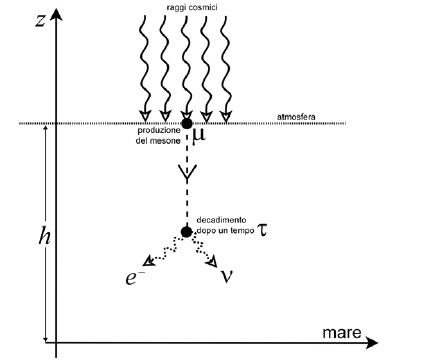
\includegraphics[scale=1]{immagini/conferme_relspec/produzione_mu}
   \caption{\label{produzione_mu}Produzione e decadimento dei mesoni $\mu$. Il mesone viene prodotto 
dall'urto dei raggi cosmici con l'atmosfera, a un'altezza $h$. Dopo un
tempo $\tau$ esso decade in un elettrone e un neutrino.}
\end{figure}

Queste particelle instabili hanno una vita media $\tau$ che è legata alla legge di decadimento
\begin{equation}
N(t) = N_0 e^{-\lambda t}
\end{equation}

con $\tau = \dfrac{1}{\lambda}$. Nell'equazione, $N(t)$ è il numero di particelle a un
istante $t$, $N_0$ è il numero di particelle iniziali.

La vita media $\tau$ può essere misurata in laboratorio (quando i mesoni
sono a riposo), valutando la porzione di popolazione iniziale che dopo un
dato tempo $t$ non è decaduta in elettroni e neutrini. 

Abbiamo quindi tutti i dati del problema: altezza $h$, velocità $v$ e vita media $\tau$.

Secondo la fisica newtoniana, lo spazio percorso dal mesone $\mu$ tra la
nascita e la morte è

\begin{equation}
s = vt 
\end{equation}

Se si inseriscono i dati, si trova che $vt < h$, cioè che $s < h$, e quindi non
dovrebbe essere possibile rilevare mesoni di origine cosmica al livello del mare.
Al contrario, tali mesoni sono rilevati.

Vogliamo quindi dare una spiegazione a questo fenomeno, usando in modo duale sia 
la dilatazione dei tempi, sia la contrazione delle lunghezze.

\subsection{Punto di vista della terra}
Dal punto di vista della terra, la spiegazione si basa sulla dilatazione dei
tempi: la vita media $\tau$ è un tempo misurato da un ``orologio interno'' del mesone.

Possiamo schematizzare la faccenda nel diagramma di figura \ref{diagramma_mu}.

\begin{figure}[htbp]
   \centering
   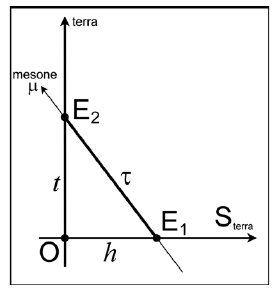
\includegraphics[scale=1]{immagini/conferme_relspec/diagramma_mu}
   \caption{\label{diagramma_mu}Diagramma spaziotemporale della vita del mesone. L'evento
$E_1$ è la produzione del mesone, l'evento $E_2$ è il suo rilevamento a terra.}
\end{figure}

Il punto fondamentale è prestare attenzione, al fine di non confondere le
misure di spazio e di tempo fatte dall'osservatore terrestre con quelle fatte dal
mesone, poichè entrambe le misure hanno valore relativo. Dato che l'esperienza 
ci dice che riusciamo a trovare mesoni al livello del mare, ribatteziamo
$\tau$ il tempo (minimo) tra la produzione e il rilevamento del mesone nel giu-
dizio del mesone. Sia invece $t$ il tempo tra gli stessi eventi nel giudizio del
laboratorio terrestre. I due eventi $E_1$ (produzione del mesone) ed $E_2$ (rileva-
mento del mesone) avvengono sulla linea di universo del mesone, quindi $\tau$ è
il tempo proprio. Per la dilatazione dei tempi abbiamo che
\[ t = \gamma (v) \cdot \tau\]

Questa è stata una delle prime verifiche sperimentali della validità della Relatività
Ristretta.

La legge di moto rispetto all'osservatore terrestre\footnote{Prestiamo attenzione: 
è vero che le leggi di moto devono avere la stessa forma nel
giudizio del mesone e in quello della terra, ma dobbiamo stare attenti che in ciascuna di 
esse tutte le grandezze devono essere misurate dallo stesso osservatore. La disomogeneità
delle misure porta inevitabilmente all'invalidità delle equazioni.}
è
\[ h = vt \]
e quindi la legge corretta è:
\[ h = (\gamma (v) \cdot v) \cdot \tau \]
che è compatibile con i dati sperimentali.

Il fenomeno si spiega dunque, rispetto all'osservatore terrestre, con la
dilatazione dei tempi: sbagliavamo nel ritenere $\tau$ il tempo di vita del mesone
nel nostro giudizio; lo era nel giudizio del mesone.

\subsection{Punto di vista del mesone}
Dal punto di vista del mesone, il tempo trascorso tra gli eventi $E_1$ (produzione, 
cioè ``nascita'' del mesone) ed $E_2$ (rilevamento del mesone al livello del
mare) è proprio $\tau$, e la velocità con cui la terra precipita addosso al mesone è
sempre $v$. Dunque abbiamo ancora il paradosso che, sulla carta, dovremmo
avere:
\[ v\tau < h \]
quando invece accade il contrario. Qui non possiamo più far valere la dilatazione 
dei tempi: il tempo $\tau$ è il tempo proprio, non c'è scampo.

Il paradosso è ancora dovuto al fatto che nella legge $v\tau < h$ stiamo impiegando 
grandezze eterogenee: $\tau$ è infatti misurato dal mesone, $h$ è misurato
dalla terra. Il paradosso nasce quindi dal mischiare nella stessa equazione
del moto uniforme grandezze misurate da osservatori diversi. Se ci poniamo nel punto di vista
del mesone, dobbiamo usare il tempo $\tau$, ma anche la distanza $d$ che il
mesone attribuisce alla terra al momento della sua nascita (anche le lunghezze
sono infatti relative). La situazione è riassunta nel diagramma di figura \ref{diagramma_mu2}.

Per determinare le distanze, dobbiamo considerare l'evento $E_3$ che si trova sulla linea
di universo della terra e che è simultaneo ad $E_1$ nel giudizio del mesone.
\begin{figure}[htbp]
   \centering
   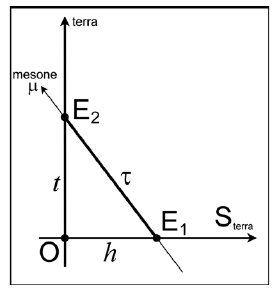
\includegraphics[scale=1]{immagini/conferme_relspec/diagramma_mu}
   \caption{\label{diagramma_mu}Diagramma spaziotemporale modificato aggiungendo il punto
di vista del mesone. In particolare, quando il mesone viene prodotto ($E_1$), nel
giudizio del mesone la terra si trova in $E_3$ . Viceversa, nel giudizio della terra,
essa si trova in $E_4$ . Quindi $k$ è la distanza tra punto di produzione e terra,
nel giudizio del mesone; $h$ è la stessa distanza nel giudizio terrestre. $\theta$ è il
parametro di rapidità.}
\end{figure}

Sia inoltre $E_4$ l'evento che avviene sulla terra contemporaneamente ad $E_1$ nel
giudizio dell'osservatore terrestre. Dal triangolo $E_1$, $E_3$, $E_4$, ricaviamo che
\[ h = d cosh \theta = \gamma(v) \cdot d \]
fatto che traduce la contrazione delle lunghezze. Quindi, nel giudizio del
mesone, la terra si trovava inizialmente a una distanza $d < h$ contratta del
fattore $cosh \theta = \gamma(v)$ rispetto alla distanza valutata dalla terra. La legge di
moto va dunque riscritta come
$d = v\tau$,
formulazione che è compatibile con i dati sperimentali.

Dunque, l'esperimento del mesone, dal punto di vista del mesone, è spiegato 
in maniera simmetrica, dalla contrazione delle lunghezze. Dilatazione
dei tempi e contrazione delle lunghezze sono perciò fenomeni duali che non
possono sussistere separatamente: l'uno implica l'altro. 

Dal punto di vista della geometria dello spaziotempo di
Minkowski, questa dualità è legata alla peculiarità delle rotazioni iperboliche
per cui, se ruota l'asse dei tempi di un osservatore, deve contemporaneamente
ruotare anche la piattaforma spaziale, in modo simmetrico rispetto al cono
luce, così da rispettare una condizione di ``perpendicolarità'' (ortogonalità) 
che ``graficamente'' è diversa dal caso euclideo.

\section{Il paradosso dei gemelli}

Consideriamo tre osservatori inerziali $A$, $B$, $C$ tali che $B$ e $C$ si muovano
rispetto ad $A$ con la stessa velocità $v$ ma da parti opposte. La situazione è
quella rappresentata in figura \ref{gemelli1}.

\begin{figure}[htbp]
   \centering
   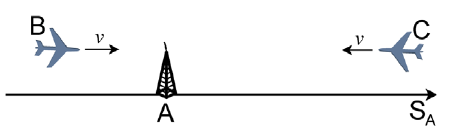
\includegraphics[scale=1]{immagini/conferme_relspec/gemelli1}
   \caption{\label{gemelli1}Situazione del paradosso dei gemelli. $B$ e $C$ si avvicinano con
velocità $v$ ad $A$; $C$ è più lontano da $A$ rispetto a $B$ (nel giudizio di $A$).}
\end{figure}

Possiamo pensare che $A$ sia la torre di controllo di un aeroporto, e che
$B$ e $C$ siano due aerei in avvicinamento. Supponiamo che, nel giudizio di $A$,
inizialmente $C$ sia molto più lontano.

\begin{figure}[htbp]
   \centering
   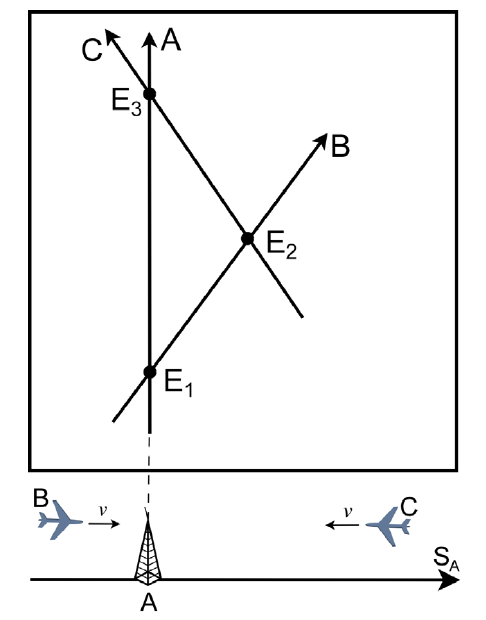
\includegraphics[scale=1]{immagini/conferme_relspec/gemelli2}
   \caption{\label{gemelli2}Situazione del paradosso dei gemelli. $B$ e $C$ si avvicinano con
velocità $v$ ad $A$; $C$ è più lontano da $A$ rispetto a $B$ (nel giudizio di $A$).}
\end{figure}

Disegnamo il diagramma spaziotemporale  e consideriamo i seguenti eventi. 
$B$ si sta avvicinando da sinistra ad $A$, sino a quando lo
incontra.
\begin{itemize}
 \item $E_1$: al tempo $t_A(E_1) = 0$ (misurato da $A$) $B$ passa per $A$, e concorda
di tarare il suo orologio in modo tale da segnare anch'esso $t_B(E_1) = 0$ (sincronizzazione degli orologi di A e B).
\end{itemize}

Poi $B$ si allontana da $A$, viaggiando verso destra, e incrocia $C$.
\begin{itemize}
\item $E_2$: $B$ incrocia $C$ che si sta avvicinando ad $A$ quando il suo orologio
segna $t_B (E2) = 1 h$ (per fissare le idee). $B$ e $C$ concordano di regolare
l'orologio di $C$ in modo tale che $t_C (E2) = 1 h$ anch'esso (sincronizzazione
degli orologi di $B$ e $C$).
\end{itemize}

Abbandoniamo ora $B$ e seguiamo $C$ nel suo avvicinamento ad A. Poiché
distanza da percorrere è (nel giudizio di $A$) la stessa di quella percorsa da $B$,
e dato che $C$ si avvicina ad $A$ con la stessa velocità con cui $B$ si allontanava,
è chiaro che $C$ ci metterà ad avvicinarsi lo stesso tempo che $B$ ci ha messo
ad allontanarsi (nel giudizio di $A$).

\begin{itemize}
\item $E_3$: $C$ passa per $A$, quando l'orologio di $C$ segnerà $t_C (E3 ) = 2h$.
\end{itemize}

La domanda paradossale è: quanto tempo è trascorso per $A$ tra gli eventi $E_1$ 
ed $E_3$?

Innanzitutto spieghiamo perchè abbiamo chiamato questo paradosso ``pa-
radosso dei gemelli''. Supponiamo che vi siano due gemelli; il primo ($A$) sta
fermo in terra nella torre di controllo di un aeroporto, il secondo invece viaggia
con velocità relativa $v$ rispetto ad $A$ e poi se ne torna indietro. Questo
gemello corrisponde all'unione di $B$ e $C$; $B$ per la fase di andata, $C$
nella fase di ritorno: è come se, incrociando $C$, $B$ ``saltasse sul suo aereo'' e
ritornasse indietro\footnote{Tutto questo è un ``trucco'' per evitare di parlare di 
accelerazioni: se il gemello $B$ dovesse invertire rotta, dovrebbe decelerare, e quindi non saremmo 
non sarebbe più un osservatore inerziale. Ci inventiamo quindi un altro
osservatore $C$ da abbinare a $B$, un osservatore che si occupi del viaggio di ritorno.}. 
Chiameremo perciò questo secondo gemello $B+C$.

Ora cerchiamo di rispondere alla domanda precedente: appurato che per
il gemello $B + C$ tra gli eventi $E_1$ ed $E_3$ sono trascorse due ore, quanto tempo
è trascorso per il gemello $A$ tra gli stessi eventi? 

\begin{figure}[htbp]
   \centering
   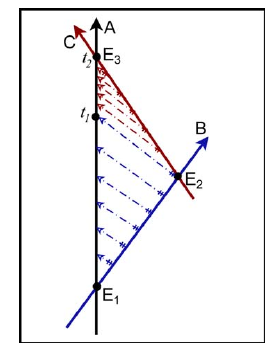
\includegraphics[scale=1]{immagini/conferme_relspec/radargemelli.png}
   \caption{\label{radar_gemelli}Il metodo radar.}
\end{figure}

Rispondiamo alla domanda facedo uso del metodo radar spiegato sopra e illustrato 
in \ref{radar_gemelli}.

Per confrontare i tempi trascorsi usiamo il metodo dello scambio di segnali
luminosi (metodo che sta alla base della geometria di Minkowski). Suppo-
niamo che, mentre si allontana, $B$ invii $n$ segnali luminosi con periodo $T$
(ad esempio, $n = 6$ e $T = 10 \min$, per fissare le idee). L'ultimo segnale ar-
riva ad $A$ al suo tempo $t_1$ . Supponiamo poi che $C$ faccia la stessa cosa nel
suo avvicinarsi ad $A$: anch'esso invierà $n$ segnali con periodo $T$ , l'ultimo dei
quali è scambiato quando $C$ incrocia $A$, al tempo $t_2$ nel giudizio di $A$ (con
riferimento ancora alla figura \ref{radar_gemelli}).
Il tempo totale trascorso per il gemello $B + C$ è la somma dei periodi di
emissione dei segnali luminosi. Il tempo totale trascorso per $A$ è invece la
somma dei periodi di ricezione. Scindiamo le due diverse fasi.
Durante l'allontanamento di $B$ si ha che
\begin{equation}
T_{ric} = k \cdot T_{emiss} = kT 
\end{equation}

e dunque
\begin{equation}
 t_1 = nT_{ric} = kn \cdot T_{emiss} = knT = kT_B
\end{equation}
ove $T_B$ è la durata del tempo di viaggio di $B$.

Durante l'avvicinamento di $C$ si ha che
\begin{equation}
T_{ric} = \frac{1}{k} T_{emiss}
\end{equation}

e dunque
\begin{equation}
t_2 - t_1 = n T_{ric} = \frac{n}{k} T_{emiss} = = \frac{n}{k} T_{C}  
\end{equation}

ove $T_C$ è la durata del tempo di viaggio di $C$.

Dato che, per simmetria, i due tempi di viaggio di $B$ e $C$ devono essere
uguali, $T_B$ = $T_C$ , ricaviamo che:

\begin{equation}
\begin{split}
t_2 &= t_1 + (t_2 - t_1 ) = kT_B + k^{-1} T_C = (k + k ^{- 1})T_B = \frac{1}{2}(k + k^{- 1})2 T_B = \\
&= \frac{1}{2} (k + k^{-1})(T_B + T_C ) = \gamma(v) \cdot (T_B + T_C )
\end{split}
\end{equation}

Dunque il tempo totale trascorso per $A$ è $\gamma(v)$ volte la somma dei tempi
trascorsi per $B$ e per $C$, cioè $\gamma(v)$ volte il tempo totale trascorso per il
gemello $B + C$. Evidentemente, i due tempi coincidono solo se $v = 0$; ne
concludiamo che il gemello $A$ (che non si è allontanato) è invecchiato di più
rispetto all'altro gemello $B + C$.

Nasce però un'obiezione sensata: questa conclusione sembra violare il Principio di Relatività!
Il moto è infatti relativo, quindi non si può dire se sia
il gemello $B + C$ ad allontanarsi da $A$ o se sia invece $A$ che si allontana a
sinistra da $B + C$ e poi si riavvicina. Se le due situazioni sono indistinguibili,
allora gli effetti devono essere uguali, e perciò $B + C$ deve invecchiare più di
$A$! C'è una contraddizione logica nella geometria di Minkowski? Quindi la
geometria di Minkowski non sta in piedi? Dove sta l'inghippo?
Sia $A$ sia $B + C$ vedono accadere $E_1$ ed $E_3$ nello stesso luogo, ma tra
questi due gemelli c'è una differenza fondamentale: uno dei due non è un
vero e proprio osservatore inerziale, o meglio, c'è un istante in cui egli cessa
di essere un osservatore inerziale. Il punto chiave è l'inversione del moto:
nel punto di inversione del moto, il gemello $B + C$ smette infatti per un
attimo di essere inerziale: i suoi pendoli e i suoi giroscopi impazziranno,
onde poi riprendere il normale comportamento nella fase di ritorno. Questa
differenza che pare microscopica, è in realtà assai significativa: $A$ è sempre
un osservatore inerziale, $B + C$, per un pur breve istante, non lo è.

La risposta è quindi che la situazione non è simmetrica. Per rimanere nel
campo degli osservatori inerziali dobbiamo confrontare $A$ con due osservatori
($B$ e $C$), situazione palesemente asimmetrica! 
Stiamo quindi confrontando un osservatore inerziale con un osservatore
non inerziale, e perciò non possiamo invocare il Principio di Relatività.

\begin{figure}[htbp]
   \centering
   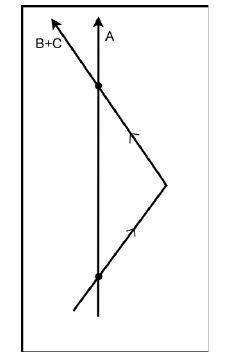
\includegraphics[scale=1]{immagini/conferme_relspec/dis_triang_mink.png}
   \caption{\label{dis_triang_mink}La disuguaglianza triangolare nello spaziotempo di Minkowski è invertita.}
\end{figure}

Nella geometria di Minkowski, questa asimmetria si manifesta nel fatto
che confrontiamo un segmento del genere tempo (quello di $A$) con una spezzata
del genere tempo (quella di $B+C$) - v. fig. \ref{dis_triang_mink}. Abbiamo quindi trovato
che nella geometria di Minkowski, per triangoli del genere tempo, vale la disuguaglianza
triangolare invertita: un lato è maggiore o uguale della somma
degli altri due lati. 

Questo è il significato geometrico del paradosso dei gemelli. 
Da questo punto di vista, tale paradosso non è altro che lo studio
della geometria di un triangolo del genere tempo in $M$ e la scoperta della
disuguaglianza triangolare invertita.


\begin{figure}[htbp]
   \centering
   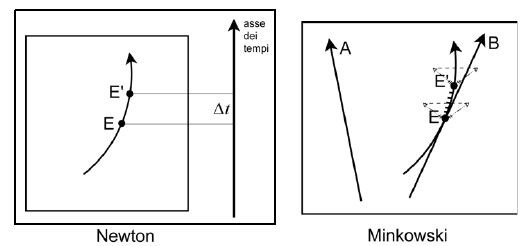
\includegraphics[scale=1]{immagini/conferme_relspec/tempi.png}
   \caption{\label{tempi}Differenza nella concezione degli intervalli di tempo tra lo 
schema classico e lo spaziotempo di Minkowski. Nello spaziotempo newtoniano le durate hanno carattere assoluto. 
Nello schema minkowskiano, le durate sono lunghezze d'arco, dipendono dal percorso.}
\end{figure}

Il paradosso dei gemelli ci fa capire la natura del tempo relativistico: il tempo è una lunghezza d'arco,
ovvero le durate dipendo dal percorso, esattamente come lo spazio percorso.

\subsection{Esperimento di Hafele-Keating}

Nel 1972 si è avuta la prima verifica sperimentale del paradosso dei gemelli
fuori dai laboratori, con l'esperimento di Hafele-Keating. Essi hanno preso
tre orologi atomici identici, ne hanno lasciato uno a terra (a Baltimora) e
hanno posto gli altri due in volo su aerei di linea, lanciati in versi opposti a
fare il giro equatoriale della terra\footnote{L'utilizzo di due aerei in luogo di uno solo è
per ovviare ad alcuni effetti gravitazionali inevitabilmente presenti e dovuti alla rotazione terrestre.}.

Ciò costringe i tre orologi a percorrere tre linee di universo diverse nello spaziotempo, 
ma avendo due eventi coincidenti: l'evento $E_0$ di partenza di due aerei e l'evento $E_1$ di ritrovo dei tre orologi
dopo il giro del mondo degli aerei.

\begin{figure}[htbp]
   \centering
   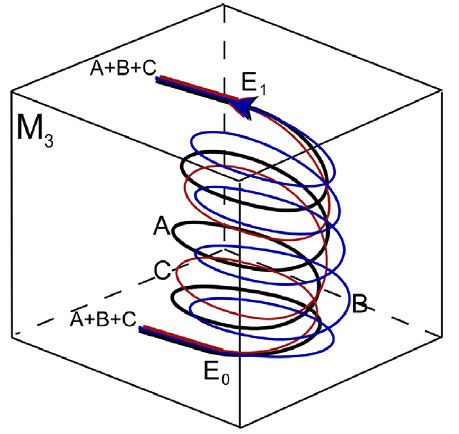
\includegraphics[scale=1]{immagini/conferme_relspec/hafele_keating.png}
   \caption{\label{hafele_keating} Esperimento di Hafele-Keating. $A$ (linea nera) è l'orologio
fermo a Baltimora; $B$ è l'orologio collocato sull'aereo in viaggio equatoriale
nello senso di rotazione terrestre. $C$ è l'orologio collocato sull'aereo in viaggio
in verso contrario rispetto al senso di rotazione terrestre. Tutte le linee di
universo sono, in prima approssimazione eliche cilindriche. Prima di $E_0$ (par-
tenza) e dopo $E_1$ (ritrovo) esse coincidono completamente. Tra i due eventi, le
eliche degli osservatori hanno passi diversi. La differenza dei percorsi fatti da
$A$, $B$ e $C$ tra $E_0$ ed $E_1$ si ripercuote in una differenza di cammino percorso, ma
anche di tempo trascorso - essendo il tempo in tutto e per tutto una lunghezza
d'arco, esso dipende infatti dal cammino di integrazione.}
\end{figure}

La figura \ref{hafele_keating} riporta le linee di universo di tali orologi in uno spazio
bidimensionale (supponiamo che lo spazio sia la sezione terrestre, tagliata
equatorialmente con il piano su cui circolano ambedue gli aerei in moto). Sia
$A$ l'orologio dermo a Baltimora, siano $B$ e $C$ gli orologi in viaggio sugli aerei.
$A$ non è inerziale, si muove con la rotazione terrestre. Per quanto riguarda
gli orologi $B$ e $C$, anche le loro linee di universo saranno eliche cilindriche,
ma aventi passi diversi, strutturate in modo diverso. Ciò che accomuna le tre
linee di universo è il fatto che esse differiscono solamente nei tratti compresi
tra gli eventi $E_0$ ed $E_1$ : prima della partenza e dopo l'arrivo, infatti, i tre
orologi sono tutti situati a Baltimora, nel medesimo luogo, ove ritornano alla
fine del viaggio.
Nella figura \ref{hafele_grafico} si può vedere come l'effetto risulti evidente dai
dati sperimentali.
Il fatto significativo è che nel tratto in cui le tre linee si distinguono,
i tre orologi battono diversamente: all'arrivo a Baltimora, gli orologi $B$ e
$C$ in viaggio hanno battuto più lentamente, e segnano di conseguenza un
tempo leggermente inferiore all'orologio $A$, sempre solidale con la terra -
una differenza leggera, ma rilevabile e rilevata dall'esperimento. Se al posto
dell'orologio e degli aerei, avessimo tre macchine e tre contachilometri non ci
stupiremmo affatto di questo risultato: ci sembrerebbe assai naturale che le
tre auto, partite da $E_0$ , giunte a $E_1$ tramite percorsi diversi, abbiano percorso
un diverso numero di chilometri. Questo accade in maniera del tutto analoga
anche per i tempi, poichè il tempo nello spaziotempo di Minkowski è una
lunghezza d'arco, e come tale va trattata. Integrando su cammini diversi,
otteniamo risultati diversi.
\begin{figure}[htbp]
   \centering
   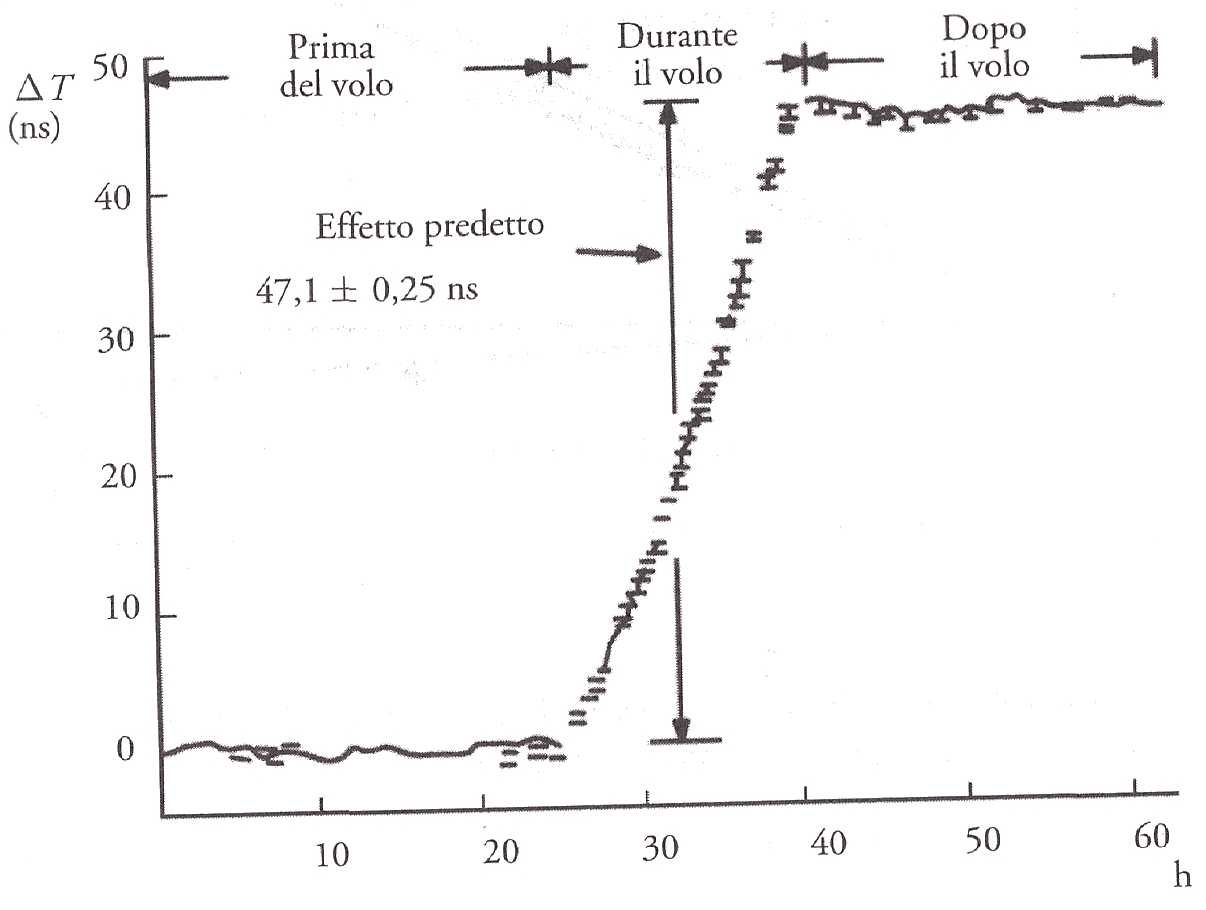
\includegraphics[scale=0.2]{immagini/conferme_relspec/hafele_grafico}
   \caption{\label{hafele_grafico} Esperimento di Hafele-Keating: in ascisse è riportato il tempo
durante il quale è stata controllata la marcia degli orologi, mentre in ordinate è riportata la differenza
fra i tempi da essi marcati.}
\end{figure}